\subsection{Intro}
    \subsubsection{QS algorithm}
    \begin{definition}
        \begin{lstlisting}[language=Python, caption={Quicksort Algorithm Pseudocode with Comments}]
            Quicksort (list in, int left, int right):
                pivot = Partition(in, left, right)   # Partition the list and return the pivot 
                if (pivot > left):                  # If elements on the LS of pivot
                    Quicksort(in, left, pivot)      # Apply QS on the left partition
                if (pivot < right):                 # If elements on the RS of pivot
                    Quicksort(in, pivot + 1, right) # Apply QS on the right partition
        \end{lstlisting}
    \end{definition}

    \begin{intuition}
        \begin{itemize}
            \item \textbf{Quicksort is a divide-and-conquer algorithm:}
            \begin{itemize}
                \item The main idea is to partition the list around a \textbf{pivot element}.
                \item After partitioning, the pivot element is placed in its correct position.
            \end{itemize}
            
            \item \textbf{Steps of Quicksort:}
            \begin{itemize}
                \item \textbf{Choose a pivot element:} This can be the first element, the last element, or any random element in the array.
                \item \textbf{Partitioning:} 
                \begin{itemize}
                    \item Elements smaller than the pivot are moved to the left.
                    \item Elements larger than the pivot are moved to the right.
                \end{itemize}
                \item \textbf{Recursively apply Quicksort:}
                \begin{itemize}
                    \item Apply Quicksort to the subarray to the left of the pivot.
                    \item Apply Quicksort to the subarray to the right of the pivot.
                \end{itemize}
            \end{itemize}
            
            \item \textbf{Base case:}
            \begin{itemize}
                \item When the subarray has one or zero elements, it is already sorted, and no further partitioning is needed.
            \end{itemize}
        \end{itemize}        
    \end{intuition}

    \subsubsection{Partition}
    \begin{definition}
        \begin{lstlisting}[language=Python, caption={Partition Function Pseudocode with Comments}]
            int Partition (in, left, right):
                ls = left                        # Left pointer (starting index)
                pivot = in(left)                 # Choose the leftmost element as the pivot
                for i = left + 1 to right:       # Iterate over the rest of the elements
                    if (in(i) <= pivot):         
                        ls = ls + 1              # Increment ls to track smaller elements
                        swap(in(i), in(ls))      # Swap current element with the element at ls
                swap(in(left), in(ls))           # Place pivot element in correct position
                return ls                        # Return the index of the pivot
        \end{lstlisting}


        \customFigure[0.5]{00_Images/QS_LS.png}{Partition}
    \end{definition}

    \begin{intuition}
        \customFigure[1]{00_Images/Quicksort_Example1.png}{Quicksort example.}          
    \end{intuition}

\subsection{QS basic analysis}
    \subsubsection{Best case}
    \begin{derivation}
        The array is always split exactly in half (i.e. picking the median as the pivot), leading to a balanced partition. The recurrence relation for quicksort in this scenario is:

        \begin{equation*}
            T(n) = 2T\left(\frac{n}{2}\right) + \Theta(n)
        \end{equation*}
        \begin{itemize}
            \item $T\left(\frac{n}{2}\right)$: Time to sort $n/2$ elements.
            \item $\Theta(n)$: Time for partition
        \end{itemize}

        \begin{center}
            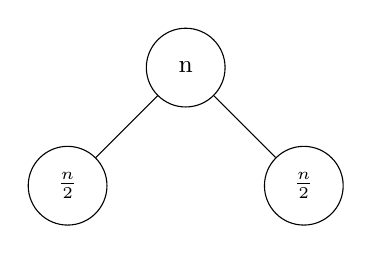
\begin{tikzpicture}[level distance=1.5cm, sibling distance=3cm, every node/.style={circle, draw, minimum size=1cm, font=\small}]
                % Root level for BC
                \node {n}
                    % First level of BC partitioning
                    child {node {$\frac{n}{2}$}}
                    child {node {$\frac{n}{2}$}};
            \end{tikzpicture}
        \end{center}

        \noindent Now using the Master Theorem:
        \begin{equation*}
        T(n) = \Theta(n \log n)
        \end{equation*}
    \end{derivation}

    \subsubsection{Worst case (informal)}
        \begin{derivation}
            The array is already sorted (or reverse sorted) and we choose the first or last element as the pivot, the recurrence relation for quicksort is:

            \[
            T(n) = T(n-1) + \Theta(n)
            \]

            \begin{center}
                % Worst Case (WC) Tree
                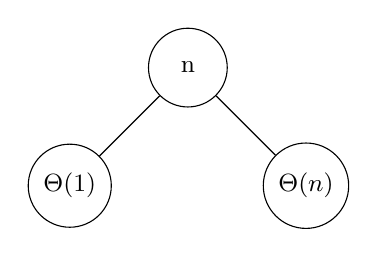
\begin{tikzpicture}[level distance=1.5cm, sibling distance=3cm, every node/.style={circle, draw, minimum size=1cm, font=\small}]
                    % Root level for WC
                    \node {n}
                        % First level of WC partitioning
                        child {node {$\Theta(1)$}}
                        child {node {$\Theta(n)$}};
                \end{tikzpicture}
            \end{center}

            \noindent This recurrence relation expands as follows:

            \begin{align*}
                T(n) &= T(n-1) + \Theta(n) \\
                    &= \left(T(n-2) + \Theta(n-1)\right) + \Theta(n) \\
                    &= \left(T(n-3) + \Theta(n-2)\right) + \Theta(n-1) + \Theta(n) \\
                    &= \cdots \\
                    &= \Theta\left(\sum_{i=1}^{n} i\right) \\
                    &= \Theta\left(\frac{n(n+1)}{2}\right) \\
                    &= \Theta(n^2)
            \end{align*}
            \begin{itemize}
                \item $\Theta(n)$: Time to partition $n$ elements.
                \item $\Theta(n-1)$: Time to partition $n-1$ elements.
                \item $\Theta(n-2)$: Time to partition $n-2$ elements.
                \item $T(n-1)$: Time to sort $n-1$ elements.
            \end{itemize}
        \end{derivation}

    \subsubsection{Expected case}
    \begin{derivation}
        In the average case, the recurrence relation for quicksort can be expressed as:

        \[
        T(n) = T\left(\frac{n}{10}\right) + T\left(\frac{9n}{10}\right) + \Theta(n)
        \]
        \begin{itemize}
            \item \textbf{Key:} Both sides are proportional to $n$.
            \item $T\left(\frac{n}{10}\right)$: Time to sort $n/10$ elements.
            \item $T\left(\frac{9n}{10}\right)$: Time to sort $9n/10$ elements.
            \item $\Theta(n)$: Time to partition $n$ elements.
        \end{itemize}

        \noindent We can visualize this with a recursion tree:

        \customFigure[0.5]{00_Images/Quicksort_Average.png}{Quicksort average case in which each level is derived by subbing in the $T(\#)$ back into the equation above.}          

        \noindent Based on the recursive tree structure and the average-case recurrence relation, we can derive the time complexity as follows:

        \[
        T(n) = h \cdot \Theta(n)
        \]

        \noindent Now, let's calculate the height \( h \) of the tree using the largest element (i.e. right sub-tree):

        \[
        \left(\frac{9}{10}\right)^h n = 1
        \]

        \[
        h = \log_{10/9}(n) 
        \]

        \noindent Substituting this back into the overall complexity:

        \begin{align*}
        T(n) &= h \cdot \Theta(n) \\
            &= \log_{10/9}(n) \cdot \Theta(n) \\
            &= \Theta(n \log n)
        \end{align*}

    \end{derivation}

    \begin{intuition}
        Another way to do the expected case is 
        \begin{center}
            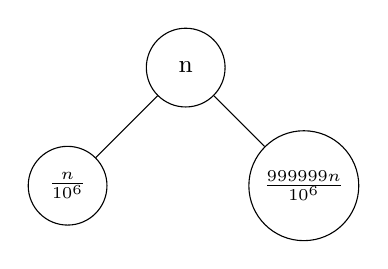
\begin{tikzpicture}[level distance=1.5cm, sibling distance=3cm, every node/.style={circle, draw, minimum size=1cm, font=\small}]
                % Root level
                \node {n}
                    % First level of partitioning
                    child {node {$\frac{n}{10^6}$}}
                    child {node {$\frac{999999n}{10^6}$}};
            \end{tikzpicture}
        \end{center}
        
        \noindent In this example, the array of size \( n \) is split into highly unbalanced sub-arrays:
        \begin{itemize}
            \item One sub-array is \( \frac{n}{10^6} \), very small compared to \( n \).
            \item The other sub-array is \( \frac{999999n}{10^6} \), almost the entire size of \( n \).
        \end{itemize}
        \vspace{1em}

        \textbf{Key:} Both cases represent different ways of dividing the input array in the Quicksort algorithm. Even though the specific subarray sizes differ in each approach, the fundamental property of the algorithm — that it breaks the problem down recursively and performs $\Theta(n)$ work at each level.
    \end{intuition}

\subsection{Worst-case (formal)}
    \begin{derivation}
        The worst-case recurrence relation for quicksort can be expressed as:

        \[
        T(n) = \text{time to QS n-elements} = \max_{1 \leq q \leq n-1} \{ T(q) + T(n-q) \} + \Theta(n)
        \]

        \begin{center}
            % Worst Case (WC) Tree
            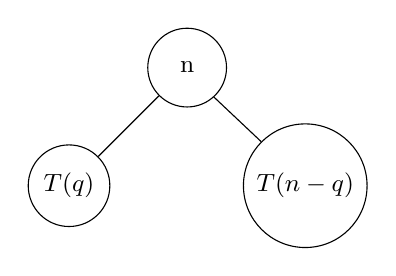
\begin{tikzpicture}[level distance=1.5cm, sibling distance=3cm, every node/.style={circle, draw, minimum size=1cm, font=\small}]
                % Root level for WC
                \node {n}
                    % First level of WC partitioning
                    child {node {$T(q)$}}
                    child {node {$T(n-q)$}};
            \end{tikzpicture}
        \end{center}

        % STOPPED HERE.
        \noindent We use substitution to show that \( T(n) \leq cn^2 \) for some constant \( c \).
        \begin{enumerate}
            \item Guess \( T(n) \leq cn^2 \).
            \item 
        \end{enumerate}
        \begin{align*}
            T(n) &\leq \max_{1 \leq q \leq n-1} \left\{ cq^2 + c(n-q)^2 \right\} + \Theta(n) \quad \text{(Achieves max at } q = 1 \text{ or } q = n-1 \text{)} \\
                 &= c \max_{1 \leq q \leq n-1} \left\{ q^2 + (n-q)^2 \right\} + \Theta(n) \quad \text{(As second derivative is positive (i.e. monotonic), plug } q = 1 \text{)} \\
                 &\leq cn^2 - 2c(n-1) + \Theta(n) \quad \text{(We can pick a large } c \text{ so that } 2c(n-1) \text{ dominates } \Theta(n)) \\
                 &\leq cn^2
        \end{align*}

        \noindent Therefore, using the substitution method, we can show that \( T(n) \leq cn^2 \), confirming that the worst-case time complexity of the quicksort algorithm is \( O(n^2) \).
    \end{derivation}

\subsection{Average-case (formal)}
    \begin{derivation}
        \[
        T(n) = \frac{1}{n} \left( T(1) + T(n-1) + \sum_{z=1}^{n-1} T(z) + T(n-z) \right) + \Theta(n)
        \]

        \begin{itemize}
            \item \textbf{Pivot Small:} $\frac{1}{n} (T(1) + T(n-1)) \leq (\Theta(n^2) + \Theta(1)) \cdot \frac{1}{n} \leq \Theta(n)$
            
            \item \textbf{There are this many elements smaller than the pivot:} $\sum_{z=1}^{n-1} T(z) + T(n-z)$
            
            \item \textbf{Got rid of \( T(1) + T(n-1) \).}
        \end{itemize}
        \vspace{1em}

        Therefore,
        \[
        T(n) \leq \frac{1}{n} \left[ \sum_{q=1}^{n-1} T(q) + T(n-q) \right] + \Theta(n) = \frac{2}{n} \sum_{k=1}^{n-1} T(k) + \Theta(n)
        \]
        \vspace{1em}

        \textbf{Use substitution to prove \( T(n) = a \log(n) + b \) for proper \( a \), \( b \).}
        \begin{enumerate}
            \item Prove the lemma $\sum_{k=1}^{n-1} k \log(k) \leq \frac{1}{2} n^2 \log(n) - \frac{1}{8} n^2$
            \begin{align*}
                \sum_{k=1}^{n-1} k \log(k) &\leq \sum_{k=1}^{\left\lfloor \frac{n}{2} \right\rfloor-1} k \log(k) + \sum_{k=\left\lceil \frac{n}{2} \right\rceil}^{n-1} k \log(k) \\
                &\leq \log \left(\frac{n}{2}\right) \cdot \sum_{k=1}^{\left\lfloor \frac{n}{2} \right\rfloor-1} k + \log(n) \sum_{k=\frac{n}{2}}^{n-1} k \\
                &= \log(n) \sum_{k=1}^{n/2} k - 2 \sum_{k=1}^{n/2} k + \log(n) \sum_{k=n/2}^{n-1} k \\
                &= \log(n) \sum_{k=1}^{n-1} k - 2 \sum_{k=1}^{\left\lceil \frac{n}{2} \right\rceil-1} k \\
                &\leq \frac{1}{2}n(n-1) \log(n) - \frac{1}{2} \left(\frac{n}{2} - 1\right) \cdot \frac{n}{2} \\
                &\leq \frac{1}{2} n^2 \log(n) - \frac{1}{8} n^2
            \end{align*}

            \item Prove using substitution
            \begin{align*}
                T(n) &\leq \frac{2}{n} \sum_{k=1}^{n-1} a k \log(k) + b + \Theta(n) \\
                &\leq a \log(n) - \frac{a}{4n} + 2b + \Theta(n) \\
                &= a n \log(n) + b + \left[\Theta(n) + b - \frac{a}{n} \right] \quad \text{ for large a}
                &\leq an \log(n) + b
            \end{align*}
        \end{enumerate}
    \end{derivation}

\subsection{Randomized QS} 
    \subsubsection{Motivation for randomized QS}
    \begin{intuition}
        \begin{itemize}
            \item Avoiding worst-case scenarios
            \item Ensuring balanced splits
            \item Works against sorted and reverse sorted arrays.
        \end{itemize}
    \end{intuition}

    \subsubsection{Random partition}
    \begin{definition}
        \begin{lstlisting}[language=Python, caption={Rand-Partition Function Pseudocode}]
            Rand-Partition (list in, left, right)
                i = random(left, right)
                swap(in(left), in(i))
                return Partition(in, left, right)
        \end{lstlisting}
        \begin{itemize}
            \item \textbf{Note:} This partition will be used to find the pivot instead in QS as it will swap random elements.
        \end{itemize}
    \end{definition}

    \subsubsection{Random partition QS}
    \begin{definition}
        \begin{lstlisting}[language=Python, caption={QuickSort with Random Partition}]
            def QS(C):
                pivot = RAND_partition(C)
                
                if pivot > left:
                    QS(C[left : pivot])
                    
                if pivot < left:
                    QS(C[pivot : right])
            \end{lstlisting}            
    \end{definition}

